\documentclass[a4paper,11pt]{article}
\usepackage{amsmath,amsthm,amsfonts,amssymb,amscd,amstext,vmargin,graphics,graphicx,tabularx,multicol} 
\usepackage[francais]{babel}
\usepackage[utf8]{inputenc}  
\usepackage[T1]{fontenc} 
\usepackage{pstricks-add,tikz,tkz-tab,variations}
\usepackage[autolanguage,np]{numprint} 

\setmarginsrb{1.5cm}{0.5cm}{1cm}{0.5cm}{0cm}{0cm}{0cm}{0cm} %Gauche, haut, droite, haut
\newcounter{numexo}
\newcommand{\exo}[1]{\stepcounter{numexo}\noindent{\bf Exercice~\thenumexo} : \marginpar{\hfill /#1}}
\reversemarginpar


\newcounter{enumtabi}
\newcounter{enumtaba}
\newcommand{\q}{\stepcounter{enumtabi} \theenumtabi.  }
\newcommand{\qa}{\stepcounter{enumtaba} (\alph{enumtaba}) }
\newcommand{\initq}{\setcounter{enumtabi}{0}}
\newcommand{\initqa}{\setcounter{enumtaba}{0}}

\newcommand{\be}{\begin{enumerate}}
\newcommand{\ee}{\end{enumerate}}
\newcommand{\bi}{\begin{itemize}}
\newcommand{\ei}{\end{itemize}}
\newcommand{\bp}{\begin{pspicture*}}
\newcommand{\ep}{\end{pspicture*}}
\newcommand{\bt}{\begin{tabular}}
\newcommand{\et}{\end{tabular}}
\renewcommand{\tabularxcolumn}[1]{>{\centering}m{#1}} %(colonne m{} centrée, au lieu de p par défault) 
\newcommand{\tnl}{\tabularnewline}

\newcommand{\bmul}[1]{\begin{multicols}{#1}}
\newcommand{\emul}{\end{multicols}}

\newcommand{\trait}{\noindent \rule{\linewidth}{0.2mm}}
\newcommand{\hs}[1]{\hspace{#1}}
\newcommand{\vs}[1]{\vspace{#1}}

\newcommand{\N}{\mathbb{N}}
\newcommand{\Z}{\mathbb{Z}}
\newcommand{\R}{\mathbb{R}}
\newcommand{\C}{\mathbb{C}}
\newcommand{\Dcal}{\mathcal{D}}
\newcommand{\Ccal}{\mathcal{C}}
\newcommand{\mc}{\mathcal}

\newcommand{\vect}[1]{\overrightarrow{#1}}
\newcommand{\ds}{\displaystyle}
\newcommand{\eq}{\quad \Leftrightarrow \quad}
\newcommand{\vecti}{\vec{\imath}}
\newcommand{\vectj}{\vec{\jmath}}
\newcommand{\Oij}{(O;\vec{\imath}, \vec{\jmath})}
\newcommand{\OIJ}{(O;I,J)}


\newcommand{\reponse}[1][1]{%
\multido{}{#1}{\makebox[\linewidth]{\rule[0pt]{0pt}{20pt}\dotfill}
}}

\newcommand{\titre}[5] 
% #1: titre #2: haut gauche #3: bas gauche #4: haut droite #5: bas droite
{
\noindent #2 \hfill #4 \\
#3 \hfill #5

\vspace{-1.6cm}

\begin{center}\rule{6cm}{0.5mm}\end{center}
\vspace{0.2cm}
\begin{center}{\large{\textbf{#1}}}\end{center}
\begin{center}\rule{6cm}{0.5mm}\end{center}
}



\begin{document}
\pagestyle{empty}
\titre{Contrôle 2}{Nom :}{Prénom :}{Classe}{Date}


\vspace*{0.5cm}
\begin{flushleft}
\begin{tabular}{|m{9.5cm}|m{1.25cm}|m{1.25cm}|m{1.25cm}|m{1.25cm}|m{1.25cm}|}
\hline 
\textbf{Compétences} & \begin{center}
\textbf{N.E.}
\end{center} & \begin{center}
\textbf{M.I.}
\end{center} & \begin{center}
\textbf{M.F.}
\end{center}  & \begin{center}
\textbf{M.S.}
\end{center} & \begin{center}
\textbf{T.B.M.}
\end{center} \\ 
\hline 
Je dois savoir reconnaitre et distinguer des problèmes relevant de situations additives et multiplicatives &  &  & & &\\
\hline 
Je dois savoir multiplier des nombres décimaux  &  &  & & &\\
\hline
Je dois savoir en géométrie, passer progressivement de la perception au contrôle par les instruments pour amorcer des raisonnements s'appuyant uniquement sur des propriétés des figures et sur des relations entre objets &  &  & & &\\
\hline 



\end{tabular} 
\end{flushleft}

\textit{N.E = Non évalué ; M.I. = Maîtrise insuffisante ; M.F. = Maîtrise fragile ; M.S. = Maîtrise satisfaisante ; T.B.M. = Très bonne maîtrise}\\


\vspace*{0.5cm}



Les exercices avec le symbole 
\includegraphics[scale=0.4]{trefle.eps}  sont à faire directement sur le sujet. Les autres se font sur la copie double.\\

\vspace*{0.5cm}

\exo{3} Poser et effectuer les opérations suivantes :               

\bmul{3}


294,75 + 4 367,538 \\


\columnbreak

213,9 - 86,23\\

\columnbreak



$42,78 \times 9,6$\\
	



\emul

\vspace*{0.5cm}



\exo{3} Calculer astucieusement en détaillant les étapes de calculs.\\



G = 1,4 + 75 + 18.60 + 125 \\



 R = 5,125 + 21 + 4,7 + 9 + 2,3 + 0,875 + 34\\




$K = 500 \times 12,39 \times 2$\\



\exo{3}\\
Angèle et Élise ont reçu chacune la même somme d'argent de leur grand-mère.\\
Angèle, qui possédait 34,65 euros, a maintenant 100 euros. \\
Élise, quant à elle, possédait 48,50 euros.\\

\noindent \initq \q Combien d'argent leur grand-mère leur a-t-elle donné ? \\
\q Combien Élise a-t-elle d'argent maintenant ?\\

\vspace*{0.2cm}




\exo{2.5} Sur la figure ci-dessous, les points S, O et R sont alignés.

\begin{center}
\includegraphics[scale=0.8]{angleexo.eps} 
\end{center}

\initq \q 
\includegraphics[scale=0.4]{trefle.eps}  Tracer \textbf{sur le sujet}, la bissectrice [Ot) de l'angle $\widehat{xOy}$.\\

\q Calculer la mesure de l'angle $\widehat{yOt}$. \textbf{Une démonstration est attendue sur votre copie double.}\\

\vspace*{0.5cm}

\exo{3.5}\\

\initq \q 
\includegraphics[scale=0.4]{trefle.eps}  Reproduire \textbf{sur le sujet} la figure ci-dessous en vraie grandeur.\\
\begin{flushleft}
\includegraphics[scale=0.85]{exoangle2.eps} 
\end{flushleft}

\q Les points O, M et N sont-ils alignés ?  \textbf{Une démonstration est attendue sur votre copie double.}\\

\vspace*{1cm}



\exo{5}\\
Une famille composée des deux parents, du fils aîné Pierre, âgé de 16 ans, des deux jumelles Mathilde et Noémie, âgées de 8 ans et du petit dernier Gabin âgé de 4 ans décide de passer une semaine à la montagne.\\
La location du logement est déjà payée.\\
Pierre et son père feront du snowboard alors que les jumelles, Gabin et leur mère feront du ski. Ils doivent donc maintenant louer le matériel.\\

\initq \q	Calculer la somme totale dépensée pour le matériel de ski sachant que :\\

\textbf{Pour une journée de location :}	\hspace*{0.45cm}- une paire de skis coûte 10,50 euros ;\\
\hspace*{6.9cm}- un snowboard coûte 14,60 euros.\\

\q	Calculer la somme totale dépensée pour les forfaits permettant d'accéder aux pistes sachant que :\\

\textbf{Pour une semaine :} 	\hspace*{0.65cm}	- le forfait « adulte » et « plus de 13 ans » coûte 180 euros ;\\
\hspace*{5.1cm}- le forfait pour les enfants de 5 à 13 ans coûte 148 euros;\\
\hspace*{5cm}   	- le forfait est gratuit pour les enfants de moins de 5 ans.\\



\vspace*{0.6cm}

\exo{}Bonus\\
On cherche un nombre mystère. Pour cela on sait que :
\bi \item si on ajoute 2 au nombre mystère,
\item puis on multiplie le résultat par 4,
\item puis on enlève 2 au résultat,
\item alors le résultat est 34.
\ei
Quel est le nombre mystère ?








\end{document}
